% Software Requirements
% CS 461 - CS Senior Capstone
% Fall 2017
% Authors: Connor Christensen, Lily Shellhammer, William Buffum


\documentclass[draftclsnofoot,onecolumn,letterpaper,10pt,compsoc]{IEEEtran}

% Packaging
\usepackage{geometry}
\usepackage{hyperref}
\usepackage{titling}
\usepackage{color}
\usepackage{listings}
\usepackage{cite}
\usepackage{pdfpages}
\usepackage{xargs}                      % Use more than one optional parameter in a new commands
%\usepackage[pdftex,dvipsnames]{xcolor}  % Coloured text etc.
%
%\usepackage[colorinlistoftodos,prependcaption,textsize=tiny]{todonotes}
%\newcommandx{\note}[2][1=]{\todo[linecolor=red,backgroundcolor=red!25,bordercolor=red,#1]{#2}}

%\newcommand\question[1]{\footnote{\textcolor{red}{#1}}}

% Paper type
\geometry{letterpaper, margin=.75in}

% Title page
\title{CS 461 - CS Senior Capstone
	\\Fall 2017
	\\Software Requirements Specification
}


\author{
	Connor I. Christensen \\
	\texttt{chriconn@oregonstate.edu}
	\\
	Lily M. Shellhammer \\
	\texttt{shellhal@oregonstate.edu}
	\\
	William B. Buffum \\
	\texttt{buffumw@oregonstate.edu}
}

\begin{document}

\begin{titlingpage}
    \maketitle
    \begin{abstract}
			Ninkasi Brewing Company is using an error prone, labor intensive and outdated brewing operations management system (BOMS) to manage the brewery data produced during the fermentation process.
			Our team (BrewHops) is tasked with creating a new system as both a proof of concept about new technology, and to give them another option for storing and viewing the brewery data.
			The new application will be web-based, to be lightweight, easy to use and accessible on many devices.
			The data will be hosted in a relational database to provide stability, power and consistent usability through time.
			\\
			\textbf{Keywords:} Brewing, Operations, Management, Ninkasi
    \end{abstract}
		\pagebreak
		\tableofcontents
\end{titlingpage}

\section{Introduction}
	\subsection{Purpose}
		This document will outline the project that satisfies the requirements for Ninkasi’s new brewing operations data management system.
		This includes a detailed description of the product created and the technology utilized to build the product.
		This document is intended for a technical audience, primarily for our instructors, Kirsten Winters and Kevin McGrath, and our sponsor, Daniel Sharp.


	\subsection{Scope}

		We will develop a web application and relational database model to manage Ninkasi data.
		We will perform a cost-benefit analysis to recommend hosting system with web service provider versus hosting on Ninkasi servers.
		Database will store:
		\begin{itemize}
			\item{
				Beer type identifier
				\footnote{A unique identifier for the type of beer, generally the name of the beer}
			}
			\item{
				Batch number
			}
			\item{
				Generation (GEN)
				\footnote{This the generation of the yeast we use to ferment the beer.
				We have to track this because we limit our yeast to ~10 generations before repropagating it.}
			}
			\item{
				Dry Hop/Adjunct Type
				\footnote{This is a field that calls out the amount of hops that need to be added to the fermenter or adjunct (special ingredient) that needs to be added to the brite tank (like vanilla beans)
				It has as a status callout to track when the hops/adjuncts were added and by whom.}
			}
			\item{Hop amount}
			\item{Data on internal brewing vat (IBV) measurements}
		\end{itemize}

		IBV data points include:
		\begin{itemize}
			\item{Specific Gravity (S.G.)
				\footnote{A measure that represents the amount of sugar left in the beer. This number starts high and decreases throughtout fermentation. When it stops we move on to the next process step.}}
			\item{pH level}
			\item{Alcohol By Volume (ABV)}
			\item{Beer temperature}
		\end{itemize}

		Provided interface will allow brewers to manually insert new batch records, update incorrect data, and view existing data.
		Interface will allow Ninkasi personnel to view data using downloadable .csv files.
		We will gage adequacy of interface based on 60\% approval from Ninkasi personnel, of which Daniel Sharp must approve.
		The goal of these requirements is to stop paper tracking of information and stop use of Excel as primary data storage.
		\\
		\\
		Stretch goals include: login system and data viewing in browser (no download required).
		\\
		\\
		We are not be responsible for advanced application security or direct control of any brewing process.

	\subsection{Definitions, acronyms and abbreviations}
		Data collected by our database will be referred to as “cellaring data”.
		This means data that has been collect while cellaring beers.
		Data points include but are not limited to: beer temperature, maturation time, amount of hops and other materials added.

		BrewHops - The name of our team

		BOMS - Brewery Operations Management System


	\subsection{References}
    No references as of 10/27/2017.
	\subsection{Overview}
		In the next sections, this document outlines details on the hardware, software, and user interface requirements for our project.
		It explains what needs to be done in order to launch our minimum viable product.
		Security, functionality, and organization are explained in detail.

\section{Description}
	\subsection{Product Perspective}
		\subsubsection{System interfaces}
			Brewers will interact with our web app in the cellar.
			The web app interacts with the database and will enter data points from the brewer's entry into the form.
			If we meet our stretch goals, brewers will be able to extract Excel spreadsheets from our web app.

		\subsubsection{User interfaces}
			The user will interact with the web app through either an internet connected phone, tablet, desktop or laptop computer.
			Phones will operate almost exclusively in portrait mode.
			Apart from the occasional chart or data display, most of the use for the phone will be entering data, which benefits from a portrait layout.
			Tablets have the ability to use both portrait or landscape mode, depending on how they would like to use the device, and which method is more convenient for them.
			Desktops and laptops will work in a landscape mode.
			For big enough screens, extra space can be used to fit more functionality on one page without having to hide menu items or actions, such as extracting data from the database.
			\\
			\\
			All Ninkasi brewers use a company provided phone and most of the brewer's work will be done through that phone.
			It's important that the site be consistent between iOS and Android to increase reliability, allow brewers to help each other with problems regardless of operating system, and reduce the learning curve.
			The environment in which the brewers are working requires that the data entry system be clear, easy to see and have a forgiving interface.
			For any new hires, the system should be intuitive\footnote{60\% acceptance of interface required to be considered "intuitive"}.
			Some phones may have smaller screens or may be held at a distance, so it's important that the font be big enough, the contrast strong enough, and the input boxes take up as much space as they can so they are easy to tap and input is easy to see.
			Brewers may have water, grain dust or other materials on their hands that will interfere with the touch capabilities of the device.
			Making the interface forgiving by making buttons, input fields and any other interactive components large will reduce error and frustration.
			\\
			\\
			If the system should use terminology that the brewers are familiar with.
			Reports should be color coded to keep the screen from filling with text and to allow the brewers to access the data at a glance.

		\subsubsection{Hardware interfaces}
			Ninkasi has a small server in their headquarters.
			A cost-benefit analysis will determine if this server will satisfy the hardware requirements of the system.
			If it will not, we will provide recommendations for web service providers.

		\subsubsection{Software interfaces}
			The user will interact with data via a web application.
			The application will expose input forms to submit data and downloadable .csv files to view data.
			We will release the software in stages, starting with a database, then a basic web input form connected to the database, then our final minimum viable product will include downloadable .csv files.

		\subsubsection{Communications interfaces}
			Web application will not implement other interfaces.

		\subsubsection{Memory constraints}
			Currently Ninkasi has space on a single server in a back room.
			Ninkasi will quickly grow out of server space which would constrain how much data we can host there.
			If Ninkasi decides to host our database on a 3rd party cloud hosting site, the memory constraints will be those of how much space they buy.

		\subsubsection{Site adaptation requirements}
			Brewers will adapt to using our web form rather than continue implementing the system they previously used.
			They will enter data not through paper logs or emails, but only through the web app.
			Our web form will need to connect to the chosen database, which may be hosted on site on Ninkasi’s server.

	\subsection{Product functions}
		Product include development of relational database and development of web application to process and present database information.
		Brewers will input information to the database using a form on the website, and retrieve information from the database as a .csv file.

	\subsection{User characteristics}
		Brewers using the web app will have all levels of education, including PhD, MS, BS, AAS, and no college experience.
		Their technical expertise about web development and coding in general will be minimal, but they will understand how to use mobile applications, how to access websites, and how to enter data into forms.

	\subsection{Constraints}
		\subsubsection{Regulatory policies}
		Because we are creating this software from the group up and there are no previous regulations for a system like this, this section is not applicable for the BrewHops team.

		\subsubsection{Hardware limitations}
		Ninkasi has a small server that we may utilize for the database.
		If we decide not to use a third party hosting site, then the small server means there will only be the amount of free space on the server available.
		This is a not a limitation for our project so much as a limitation for any possible continuation of our project from Ninkasi.

		\subsubsection{Interfaces to other applications}
		BrewHops’ application will integrate with Tanknet.
		\footnote{Tanknet is a a hardware and software system that performs physical measurements inside brewing vats and automatically collects the data and exports it digitally}
		The web app will automatically collect temperature information from Tanknet and store it in our database.


		\subsubsection{Parallel operation}
        Our web app will allow concurrent read access and use transactions for insertions and updates.

		\subsubsection{Audit functions}
        Not applicable for BrewHops team.

		\subsubsection{Control functions}
        Not applicable for BrewHops team.

		\subsubsection{Higher-order language requirements}
        Objects and callback functionality required.

		\subsubsection{Signal handshake protocols (e.g., XON-XOFF, ACK-NACK)}
        Not applicable for BrewHops team.

		\subsubsection{Reliability requirements}
		The web app will ensure data integrity for automated data collection.
		The web app will not ensure data integrity for manual data entry.
		Our site will be accessible without wait time longer than 5 seconds 90\% of the time.
		If multiple users are using the system, it should not slow down operations on the web app by more than 3 seconds.


		\subsubsection{Criticality of the application}
		The web app is not critical to Ninkasi Brewing Company’s success, but it would save the company data entry time.
		Ninkasi already has a working system that is not online.
		Our system would improve the current system by reducing time wasted from entry error and replace their working data entry processes.


		\subsubsection{Safety and security considerations.}
		This product will be light on security, as it is an internal application and should only be accessed by verified employees in the company.
		As this is not a public facing product, malicious activity is low on our list of priorities.
		Further details are outlined under the Specific Requirements section.

	\subsection{Assumptions and dependencies}
    BrewHops team will have access to Ninkasi Brewing Company's server to deploy application.

\section{Specific requirements}
	\subsection{External interfaces}
    Included in product are as follows:
        \begin{itemize}
						\item{Database: A database will either be hosted on Ninkasi's server or through a 3rd party site.
						The input to the database will include multiple columns of cellaring data, who entered the information, and timestamps. }

            \item{Web Application:}
            The web application will consist of a website that scales/changes functionality to fit the device.

                \begin{itemize}
										\item{Mobile Phone Page: The web app will scale to fit the mobile phone, mostly in portrait mode.
										The mobile version will be used for data entry and will have minimal options in comparison with the tablet or desktop.
										Data will not be extracted in .csv files through the mobile site.}

                    \item{Tablet Page: Tablets will operate in either portrait or landscape mode and will have the form and possibly more options for data extraction.}

                    \item{Desktop/Laptop Computer Page: This page will operate in landscape mode and will have the most options of the three pages.}

                    \item{Streatch goals include the ability to extracted database info in the form of .csv files}
                \end{itemize}
        \end{itemize}

	\subsection{Functions}

		When data is being input into the database, there will be basic checks on the data.
		Information being entered that is far outside the range of expected values will prompt the user to verify that the information is indeed correct.

		Every input form will strip out all html special characters to make sure that no harmful code can be injected into the database.

		Stretch goals include:
		\begin{itemize}
			\item{Adding a login interface to verify the users before they begin using the system.}
            
            \item{Implement profile levels to differentiate permissions (admin, operator, supervisor, cellar, etc.).}
            
            \item{Track authenticated user levels in database.}

			\item{Including a time and ID stamp on the data entered in case the company needs to trace back an error to a particular time or person.}
		\end{itemize}

	\subsection{Performance requirements}
		Multiple users on the web app at once will be permitted.
		There few Ninkasi brewers who will be entering data and it will be rare to have two entering at the same time.
		We will update this part of the doc when we receive the spreadsheet format from Daniel and are able to specify what values go where.
		95\% of interactions with the web page should happen in less than 5 seconds.

	\subsection{Logical database requirements}
    \begin{itemize}
        \item{Information pulled from Master Excel Spreadsheet}
            \begin{itemize}
                \item{\textbf{Fermentation Vessel, FV}: 
                    tank fermentation is carried out in.
                }
                \item{\textbf{BEER}:
                    beer abbreviations associated with temperature profiles and dry hop recipes.
                }
                \item{\textbf{BATCH}:
                    batches are groupings of sequential brew numbers inside a particular FV\footnote{Example: if there are 5 brews of IPA with numbers 3000, 3001, 3002, 3003, and 3004 in FV7, the BATCH ID will be: IPA 3000-3005 FV7.}
                }
                \item{\textbf{Yeast Generation, GEN}:
				    the generation of the yeast we use to ferment the beer.
                }
                \item{\textbf{Vol To Ferm (BBL)}}
                \item{\textbf{Vol To Bright (BBL)}}
                \item{\textbf{BRIGHT (BRITE)}:
                    tank where beer is sent after fermentation, used to track volume of beer and associated losses.
                }
                \item{\textbf{\% Yield}:
                    normally stored onces per batch but a batch from one FV may split between two smaller brite tanks or two batches from two FVs may blend into single brite tank.
                }
                \item{\textbf{Dry Hop/Amount Type}:
                    recipe for given dry hop
                    \footnote{Example: dry hop type A = 50 lb, dry hop type B = 75 lb.}
                    \footnote{dependent on the BEER and volume in fermentation (for dry hops).}.
                }
                \item{\textbf{Amount (lb)}:
                    amount in lbs of dry hops to be added to tank.
                }
                \item{\textbf{Monitoring Points}:
                    minimally measured daily.
                }
                \begin{itemize}
                    \item{\textbf{Specific Gravity}: 
                        A measure that represents the amount of sugar left in the beer. 
                        This number starts high and decreases throughtout fermentation. 
                        When it stops we move on to the next process step
                    }
                    \item{\textbf{pH}: 
                        pH level of batch in brewing vat.
                    }
                    \item{\textbf{ABV}: Alcohol By Volumne of batch.}
                    \item{\textbf{Temp}: Temperature of batch.}
                    \item{\textbf{Action}: Action taken.}
                    \item{\textbf{By}:
                        person taking the action above.
                    }
                \end{itemize}
            \end{itemize}
        \item{Frequency of use}

            Data currently updated daily and read throughout the day.

        \item{Accessing Capabilities}

            Database will be access from database access layer of web application.
    \end{itemize}

	\subsection{Design constraints}
		Ninkasi currently has one server.
		Our job is to create, or aid in creating, a new database system.
		We can either use their existing platforms, meaning limited space, or create a database on a third party hosting site.
		Either option is limited by time, we can only implement so much of the data management throughout the timeline of this project.
		Stretch goals are to expand the database and data entry options, given we have time to do so.

		\subsubsection{Standards compliance}

		There are no standards compliance requirements for our software.

	\subsection{Software system attributes}
		\subsubsection{Reliability}

		There is room for occasional bugs given that they do not damage data or inhibit the brewery process.
		Reliability of the system is a desirable goal, but the product is not a mission critical piece of software.
		Down time would be frustrating for employees, but would not render the company useless.
		That being said, it’s a reasonable goal that the system should be up 96\% of the time\footnote{Ideally as close to 100\% of the time as possible.}.

		\subsubsection{Availability}

		The system should not require a reboot, recovery or restart.
		Stretch goals include making a daily backup of the information in the database if the system were to crash or the data were to be corrupted.

		\subsubsection{Security}

		Individuals not associated with Ninkasi Brewing Company should not have access to the system.
		As this is not a public facing product, malicious activity is low on our list of priorities.
		Stretch goals will focus on security such as providing a login interface for employees, adding time stamps for data entered, and providing an easy method to find out who was responsible for entering incorrect data or misuse of the system.
		There will be checks built into the delivered product, but those will primarily be designed for taking care of user error rather than malicious intent.

		\subsubsection{Maintainability}

		This software is designed to be a proof of concept that having a system like this would be beneficial to Ninkasi's business development.
		Therefore, maintainability is not only good as a good coding practice, but it is one of the core requirements for the project that the code be maintainable and easy for others to understand.
		\\ \\
		There should be a clear separation between the frontend and the database connections.
		Our current plan involves using a REST API structure to ensure that if someone wanted to swap out the interface, or if someone needed a new connection to the database to be made, that a new port could be opened up and accessed from that space.
		\\ \\
		For the most part, code should be broken up into discrete functions that would allow for easy unit testing in the future.
		Though unit testing is not required as a goal for this project, the ability to attach some kind of testing framework will be useful for our code.

		\subsubsection{Portability}

		This program is designed to be highly portable and the format of the product was selected specifically for that reason.
		The percentage of code and components with host-depenedent elements should be as small as possible, likely around 40\%.
		Our site will be built using web technologies that should be able to operate on any common browser such as Firefox, Chrome and Edge.
		The most dependent code we will have will be the code running the database, and that will simply depend on the confguration that the server will have.
		If someone wanted to migrate the product over to a different server, they would only have to be sure that the underlying programming language like PHP, Rails some form of SQL or other tech is installed
		\footnote{We will decide on the host technology later}.

	\subsection{Organizing the specific requirements}
		We will build a user class based system. This will allow us to separate responsibilities and functionality so individuals only have access to their required tasks. In this system, we can design it hierarchically so that managers have access to all data manipulation privileges while brewers only have read or write privileges through structure forms. As a stretch goal, manager level individuals will be able to modify user permissions as needed.
	\subsection{Comments}
\section{Appendixes}
\section{Index}

\pagebreak
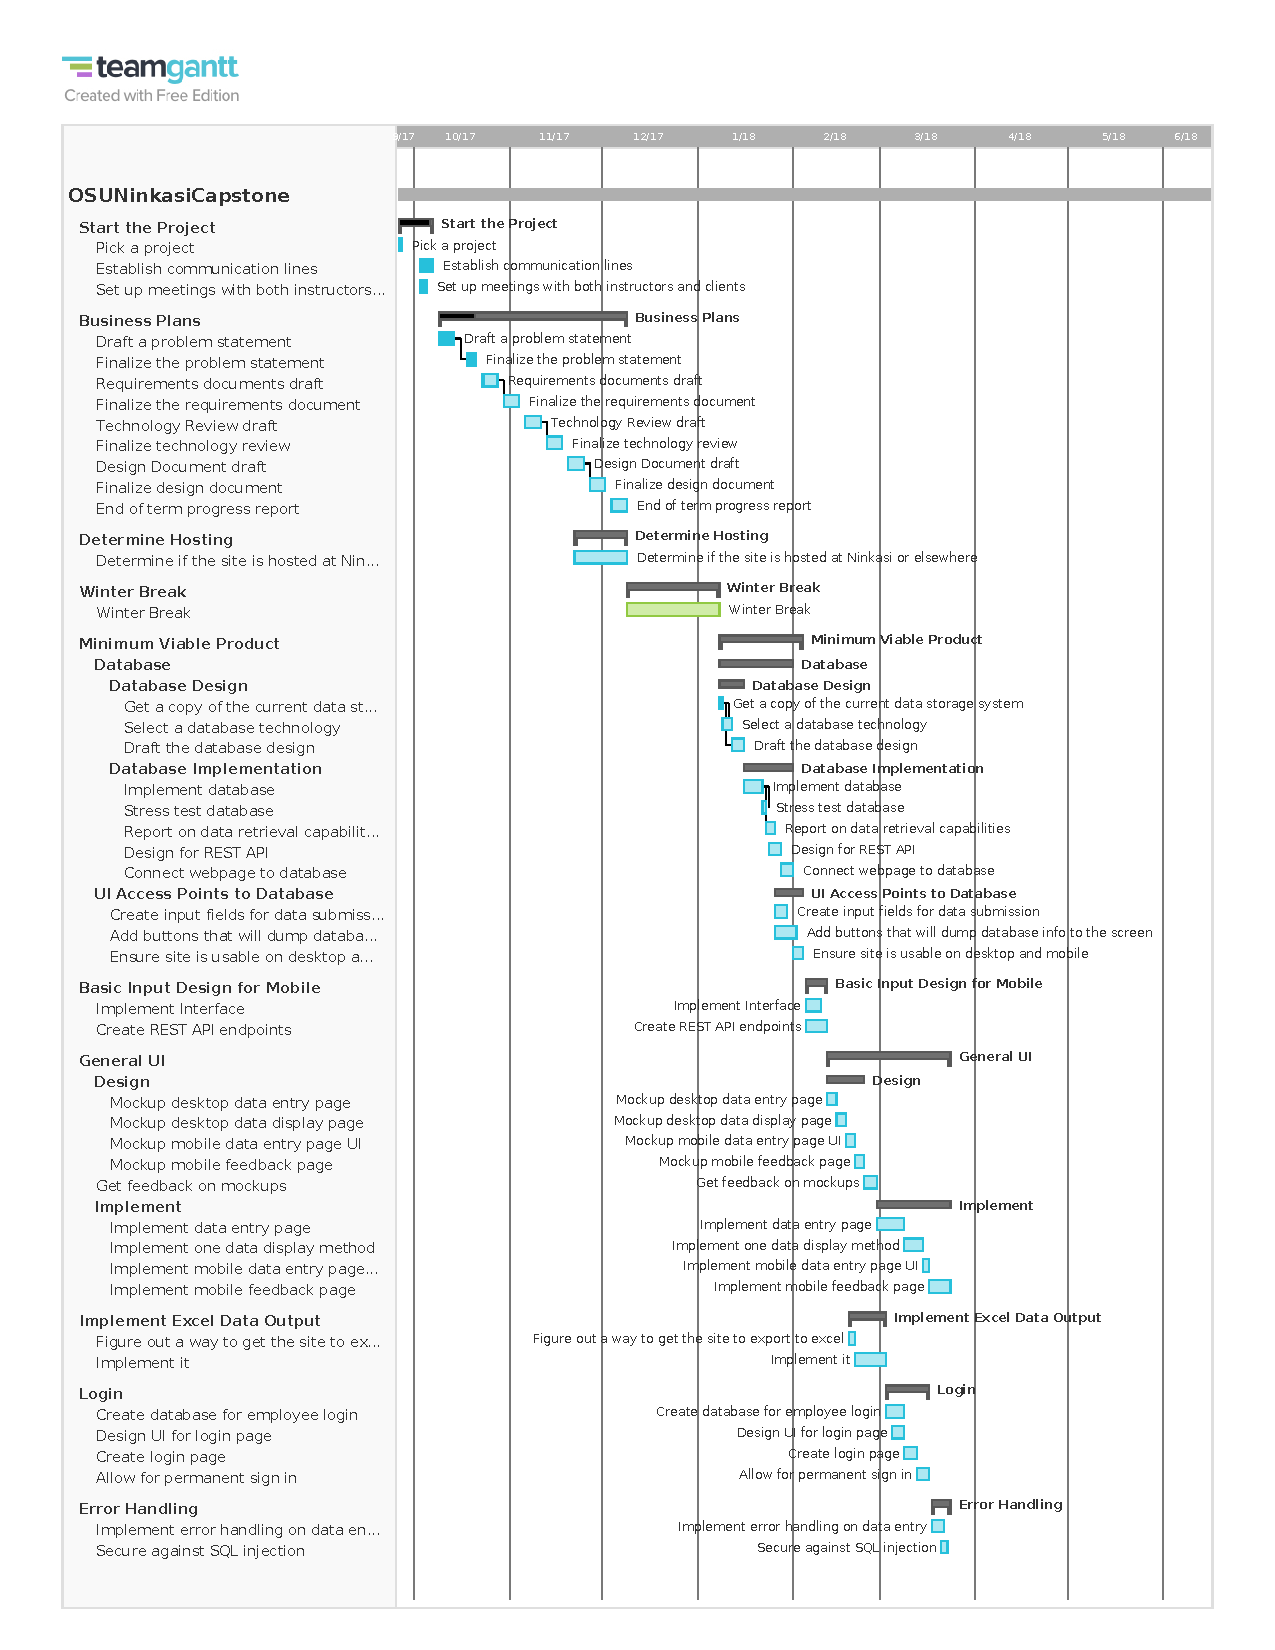
\includepdf[pages=1-2]{OSUNinkasiCapstone.pdf}

\end{document}
